% Pdf only
\documentclass[aspectratio=169]{beamer}
% For presentation
%\documentclass[aspectratio=169, notes]{beamer}
\usepackage{lmodern}
\usepackage{pgfpages}
%\setbeameroption{show notes on second screen}
%\usepackage[utf8]{inputenc} 
\usepackage[english]{babel}

%
% Choose how your presentation looks.
%
% For more themes, color themes and font themes, see:
% http://deic.uab.es/~iblanes/beamer_gallery/index_by_theme.html
%
\mode<presentation>
{
  \usetheme[]{metropolis}           % Use metropolis theme
} 

\begin{document}
\obeylines

\title[SVO SLAM implementation]{SVO SLAM implementation}
\author{Stefan Eichenberger, CPVR Lab}
\date{05.07.2019}


\begin{frame}
  \titlepage\thispagestyle{empty}
\end{frame}

\begin{frame}{Different SLAMs}
  \begin{center}
    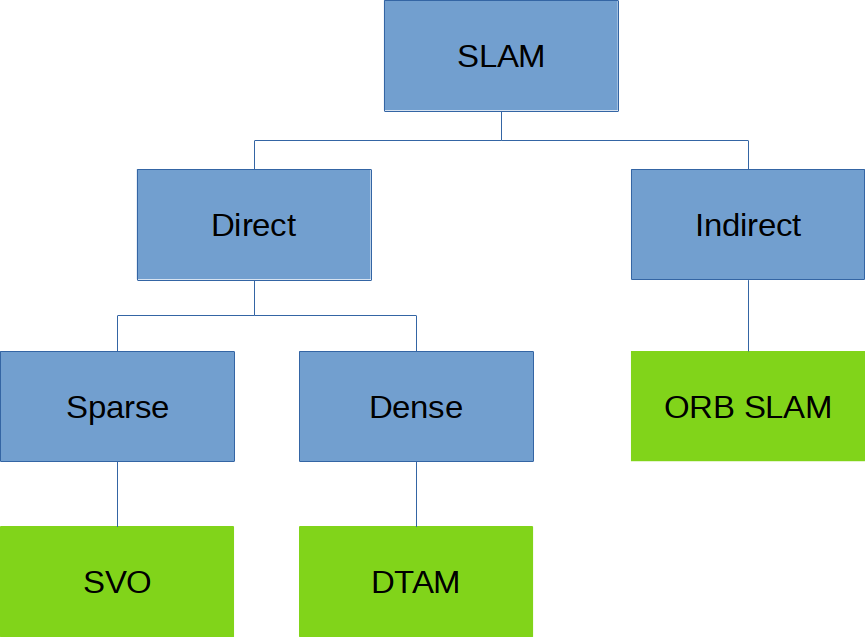
\includegraphics[height=0.9\textheight]{./img/slam_modes.png}
  \end{center}
\end{frame}

\begin{frame}{SVO SLAM}
  \begin{center}
    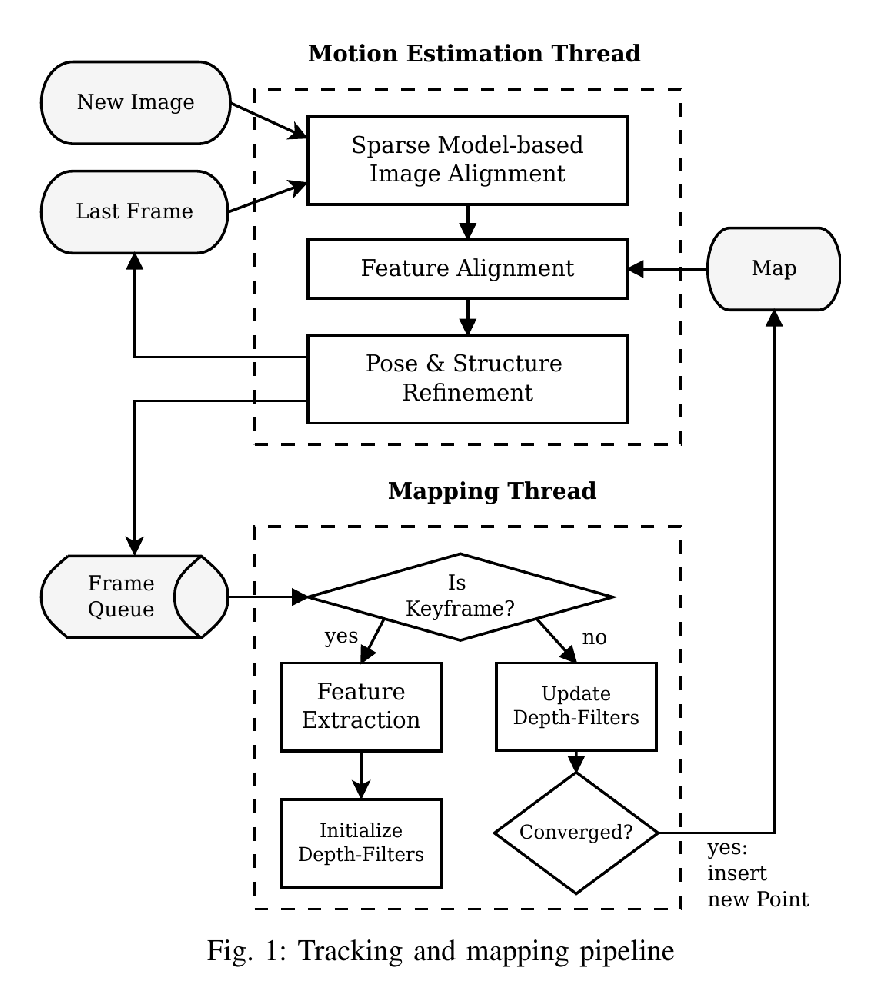
\includegraphics[height=0.9\textheight]{./img/svo_pipeline.png}
  \end{center}
\end{frame}

\begin{frame}{Current implementation}
\begin{itemize}
  \item Initial cloud from stereo camera
  \item Image to image pose alignment
  \item Image to reference refinement
  \item Pose + Cloud update based on refinement
  \item Insert new keyframe when not enough point trackable
  \item Viewer based on Websockets uses Qt3D for displaying
\end{itemize}
\end{frame}

\begin{frame}{SVO Step 1}
  \begin{center}
    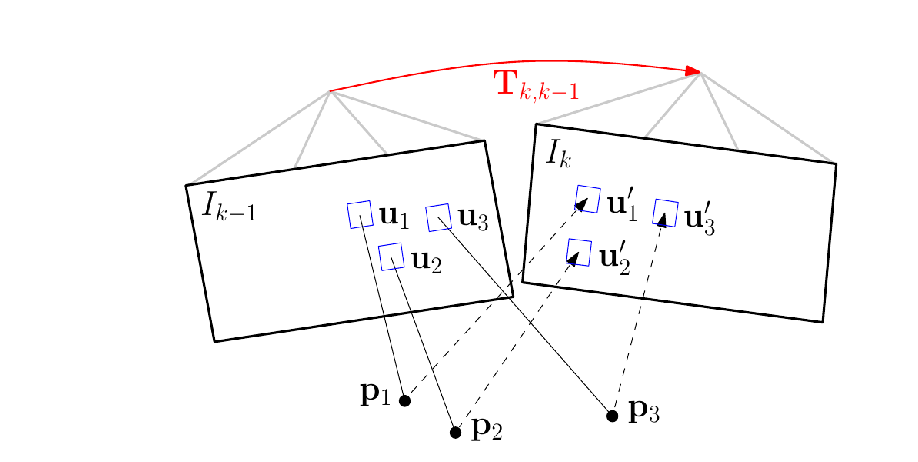
\includegraphics[height=0.9\textheight]{./img/svo_step1.png}
  \end{center}
\end{frame}

\begin{frame}{SVO Step 2}
  \begin{center}
    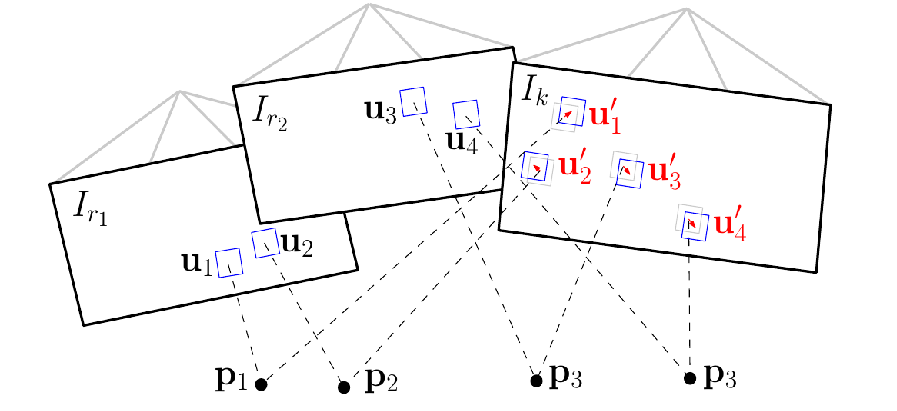
\includegraphics[height=0.9\textheight]{./img/svo_step2.png}
  \end{center}
\end{frame}

\begin{frame}{SVO Step 3}
  \begin{center}
    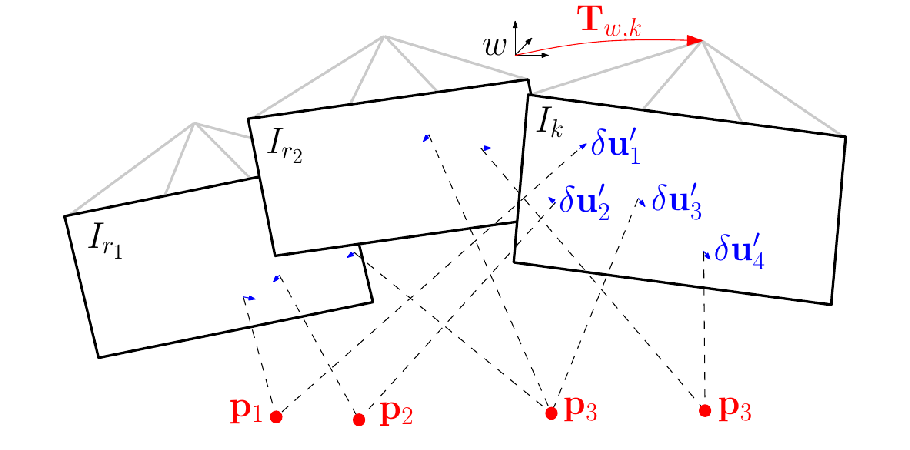
\includegraphics[height=0.9\textheight]{./img/svo_step3.png}
  \end{center}
\end{frame}

\begin{frame}{Difference to SVO}
\begin{itemize}
  \item Initial point cloud from stereo camera
  \item New keyframes do not share keypoints
  \item There is no mapping thread
\end{itemize}
\end{frame}

\begin{frame}{Depth from Stereo}
  \begin{center}
    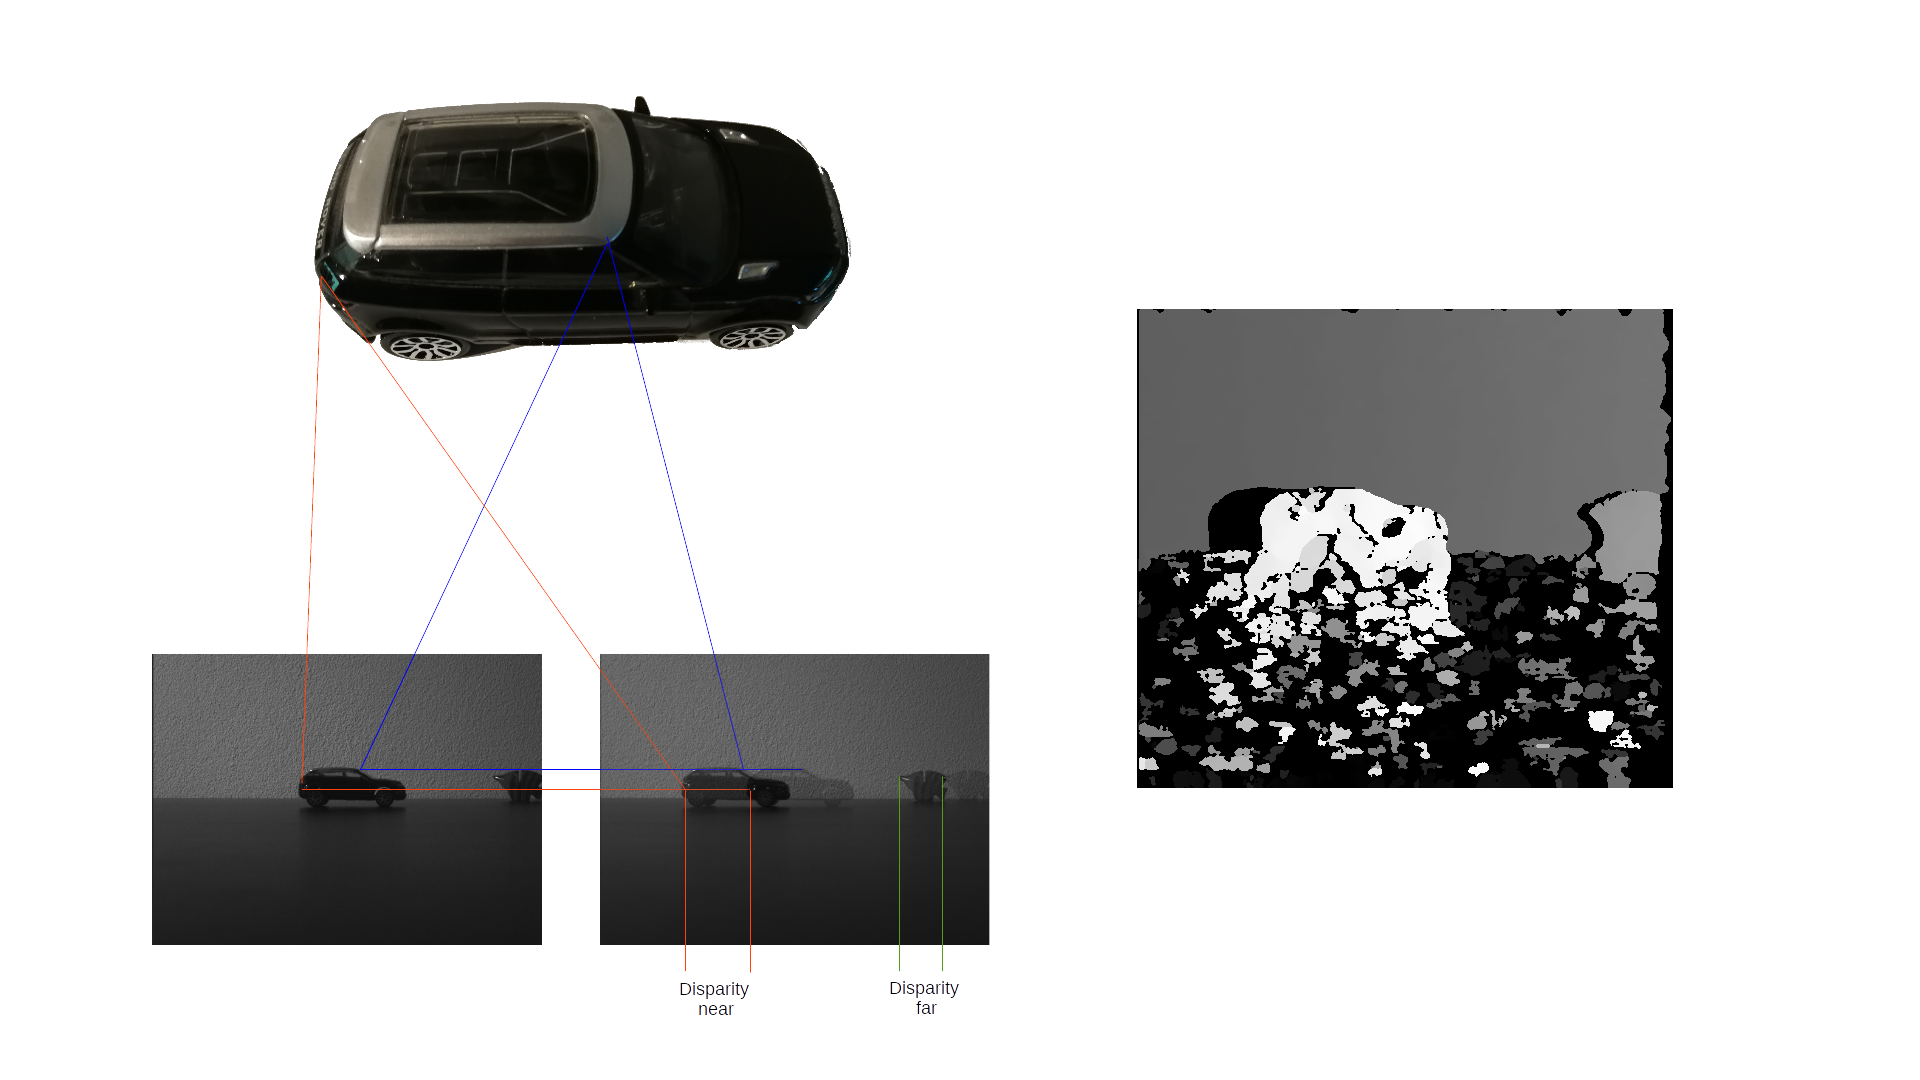
\includegraphics[height=0.9\textheight]{./img/disparity.png}
  \end{center}
\end{frame}

\begin{frame}{Planned improvements}
\begin{itemize}
  \item Move algorithm to C++ (started)
  \item Share keypoints between keyframes 
  \item Don't do rectification on image
  \item Use IMU + Kalman filter to improve motion model
  \item Add probability per point (only use likely points)
  \item Use high probability key points as vertexes for map
  \item Evaluate trajectory based on EuroC
\end{itemize}
\end{frame}


\begin{frame}{Questions}
  \begin{center}
    
\includegraphics[height=0.9\textheight]{./img/question.jpg}
  \end{center}
\end{frame}


\end{document}

